\chapter{Solución Propuesta}
\label{chap:proposal}

Un componente de considerable importancia en la composición de imágenes realistas es la iluminación. Para el cálculo de iluminación directa bajo el pipeline de renderizado estándar ya se tienen décadas de estudio y distintas técnicas que permiten tiempos de renderizado muy cortos en hardware moderno. En contraste el cálculo de iluminación indirecta sigue siendo una tarea computacionalmente compleja. 

Para el cálculo de iluminación indirecta existen varios procedimientos muchos de estos inspirados en los ya explicados en la sección \ref{sub:render_eq_procedures}. Sin embargo estos procedimientos no están pensados para renderizado en tiempo real. En la sección \ref{sec:interactive_gi_takes} examinamos algunas aproximaciones para el cálculo de iluminación indirecta en tiempo real, estas técnicas explotan ciertas características de hardware o recursos del pipeline de renderizado.

Nuestra implementación para el cálculo de iluminación global en tiempo real está fuertemente inspirada por el trabajo de Crassin y otros en 2011 \cite{CNSGE11b}. Este trabajo ya fue examinado en la sección \ref{sub:voxel_cone_tracing_orig}. La técnica fue escogida por que además de reflexión difusa también permite el cálculo de superficies lustrosas con reflexión especular a diferencia de otras técnicas como \ac{LPV} que solo permiten reflexión difusa. Una ventaja de esta aproximación es que los valores de radiancia ya se encuentran almacenados sobre una representación con vóxeles. Esto acelera el cálculo de luz incidente bajo el esquema de integración Monte Carlo visto en la sección \ref{subsec:monte_carlo_raytracing}, en este caso los conos permiten realizar una cruda aproximación de un grupo de rayos. Además de esto el algoritmo puede ser usado en escenas totalmente dinámicas.

\section{Voxelización} % (fold)
\label{sec:voxelizacion}
El trazado de conos contra geometria poligonal compleja es costoso. Encontrar los puntos de interseccion entre un cono y un poligono es mas complejo que intersecciones rayo-poligono, ademas de esto un solo cono podria intersectar muchos poligonos.

Para simplificar el trazado de conos se utiliza una discretizacion de la escena en forma de voxeles. Esta representacion puede ser filtrada a niveles mas bajos de detalle. Esto nos permite aproximar el efecto de extender la apertura del cono utilizando cada vez un nivel de detalle mas bajo a traves del recorrido del mismo.

\begin{figure}[H]
	\centering
	\begin{subfigure}[b]{.32\linewidth}
		\centering
		\captionsetup{justification=centering}
		\includegraphics[width=\linewidth]{media/finals/albedo_v256.png}
	\end{subfigure}%
	\hspace{0.01\textwidth}
	\begin{subfigure}[b]{.32\linewidth}
		\centering
		\captionsetup{justification=centering}
		\includegraphics[width=\linewidth]{media/finals/albedo_v128.png}
	\end{subfigure}%
	\hspace{0.01\textwidth}
	\begin{subfigure}[b]{.32\linewidth}
		\centering
		\captionsetup{justification=centering}
		\includegraphics[width=\linewidth]{media/finals/albedo_v64.png}
	\end{subfigure}%
	\caption{Distintos niveles de detalle de una escena voxelizada.}
	\label{fig:voxelization_details}
\end{figure}

Este proceso de voxelizacion para las partes dinamicas de la escena debe ser realizado cada vez que se realiza un cambio sobre alguna superficie que pertenece a algun objeto dinamico en la escena. Por esta razon se requiere un algoritmo de voxelizacion de alto rendimiento para mantener tiempos interactivos.

\subsection{Voxelizacion Conservativa} % (fold)
\label{sub:voxelizacion_conservativa}
Nuestra implementacion realiza voxelizacion conservativa de geometria de alto rendimiento totalmente por \ac{GPU} explotando caracteristicas del pipeline de renderizado de OpenGL. Para esto se implemento el algoritmo de voxelizacion utilizando rasterizacion en hardware explicado en el libro OpenGL Insights por Cyril Crassin y Simon Green en \empty{Octree-Based Sparse
Voxelization Using the GPU
Hardware Rasterizer} \cite{CozziRiccio12}. 

% Esta tecnica utiliza el \emph{geometry shader} y proyeccion ortogonal del triangulo por cada eje para encontrar la maxima area de voxelizacion. La voxelizacion conservativa se logra expandiendo cada vertice del triangulo segun los planos perpendiculares al triangulo por cada par de vertices del mism

Este algoritmo esta basado en el trabajo de Zhang y otros en 2007 \cite{zhang2007conservative} para la voxelization conservativa utilizando la \ac{GPU} y el trabajo de Hasselgren y otros en 2005 \cite{hasselgren2005conservative} sobre rasterizacion conservativa.

Para maximizar el area de rasterizacion la idea es proyectar cada triangulo utilizando proyeccion ortogonal por cada eje direccional. El eje dominante es escogido segun la normal del plano definido por los vertices del triangulo.

\begin{figure}[H]
	\centering
	\captionsetup{justification=centering}
	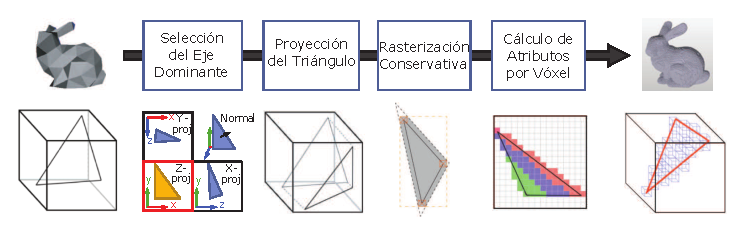
\includegraphics[width=\linewidth]{media/voxelization_pipeline.eps}
	\captaion{Pipeline de voxelizacion utilizado en nuestra implementacion.}
\end{figure}
 
Por cada triangulo proyectado es necesario generar un poligono delimitante un poco mas grande que el triangulo para garantizar la voxelizacion conservativa. Este poligono debe permitir que por cualquier triangulo proyectado tocando un pixel este va obligatoriamente a tocar el centro de este pixel por tanto el pipeline de rasterizacion generara fragmentos para este traingulo. Este poligono se genera expandiendo cada vertice del triangulo hacia afuera utilizando el \emph{geometry shader}. El poligono delimitante no sobreestima la cobertura del triangulo por tanto este no tiene forma de triangulo. Los fragmentos excedentes de este poligono son descartados en el \emph{fragment shader} utilizando un cuboide delimitante.


% subsection voxelizacion_conservativa (end)
% section voxelizacion (end)

\subsection{Voxelización Dinámica} % (fold)
\label{sub:voxelizacion_dinamica}

% subsection voxelizacion_dinamica (end)

\section{Sombreado de Vóxeles} % (fold)
\label{sec:sombreado_de_voxeles}
Para el cálculo de iluminación indirecta es necesario sombrear cada vóxel. El proceso de sombreado de vóxeles nos permite almacenar la radiancia incidente sobre la escena discretizada en vóxeles. En el trabajo de Crassin esto se hace calculando la iluminación directa sobre los vóxeles utilizando \emph{light-view maps} por cada fuente de luz como ya fue explicado en la sección \ref{subsub:voxel_capture}. Este proceso puede ser ineficiente tanto en consumo de memoria como en rendimiento cuando se considera una escena con muchas luces ya que por cada luz se debe realizar este proceso y se debe tener un mapa de luz-vista asociado (seis para luces puntuales). Otra desventaja de este método es la dependencia del rendimiento con la resolución del mapa de luz-vista. Al aumentar la resolución de esta textura también se aumenta el número de colisiones por cada fragmento que desear escribir sobre un mismo vóxel.

Nuestra implementación utiliza \emph{compute shaders} o el procesador de computo en la \ac{GPU} para el sombreado difuso de cada vóxel. Para calcular el termino difuso sobre un fragmento utilizando la \ac{BRDF} de Lambert (ecuación \ref{eq:lambert}) necesitamos saber el valor de $\rho_{d}$ el cual ya es almacenado en nuestro volumen albedo. Esta constante luego debe ser multiplicada por el $\cos(N_{x}, \Psi)$ para calcular la reflexión difusa de este fragmento. Por esto también se crea un volumen de normales. El vector $\Psi$ se obtiene a partir la dirección de cada fuente de luz en escena.

Para fuentes de luz con dirección no uniforme como luces puntuales o focales es además necesario saber la posición de este fragmento. Siendo cada vóxel una representación discreta de un espacio en escena almacenado en una textura 3D, esta posición se extrae fácilmente convirtiendo la posición tridimensional del vóxel en espacio textura a su equivalente en espacio de mundo.

Al promediar las normales en el espacio de un vóxel pueden surgir varios problemas de precisión. Esto sucede especialmente cuando un vóxel envuelve superficies finas cercanas con normales opuestas. Para solventar este problema se implementaron dos modelos de iluminación de vóxeles. El modelo de Lambert clásico utilizando la normal promedio del vóxel directamente y otro modelo al cual llamaremos Lambert Direccional Ponderado donde se calcula la reflexión difusa por cada cara del vóxel para luego promediar este resultado según el peso de cada eje en el vector normal promedio.

\begin{figure}[H]
	\centering
	\begin{subfigure}[t]{0.33\textwidth}
		\centering
		\captionsetup{justification=centering}
		\includegraphics[width=\linewidth]{media/lambert_right.png}
		\caption*{Eje x.}
	\end{subfigure}%
	\begin{subfigure}[t]{0.33\textwidth}
		\centering
		\captionsetup{justification=centering}
		\includegraphics[width=\linewidth]{media/lambert_up.png}
		\caption*{Eje y.}
	\end{subfigure}%
	\begin{subfigure}[t]{0.33\textwidth}
		\centering
		\captionsetup{justification=centering}
		\includegraphics[width=\linewidth]{media/lambert_forward.png}
		\caption*{Eje z.}
	\end{subfigure}%
	\caption{Ilustración de reflexión difusa por cada eje direccional para las caras del vóxel.}
	\label{fig:lambert_dir}
\end{figure}
% section sombreado_de_voxeles (end)

\begin{figure}[H]
	\centering
	\begin{subfigure}[t]{0.49\textwidth}
		\centering
		\captionsetup{justification=centering}
		\includegraphics[width=\linewidth]{media/classic_lambert.png}
		\caption*{Lambert..}
	\end{subfigure}%
	\hspace{0.01\textwidth}
	\begin{subfigure}[t]{0.49\textwidth}
		\centering
		\captionsetup{justification=centering}
		\includegraphics[width=\linewidth]{media/dir_lambert.png}
		\caption*{Lambert Direccional Ponderado.}
	\end{subfigure}%
	\caption{Sombreado difuso de vóxeles utilizando Lambert clásico y Lambert Direccional Ponderado. En la imagen izquierda se puede observar varios vóxeles totalmente negros, estos valores son incorrectos, causados por normales desviadas durante el proceso de voxelización. En la imagen derecha estos vóxeles ahora tienen coloración correcta. También se puede observar que objetos con normales promediadas correctamente como el piso mantienen su sombreado original en ambos modelos.}
	\label{fig:lambert_dir_diff}
\end{figure}

\subsection{Trazado y Mapeo de Sombras sobre el Volumen} % (fold)
\label{sub:trazado_de_sombras_sobre_el_volumen}

Para obtener resultados coherentes durante el trazado de conos es también necesario ocluir los voxeles con sombras generadas a partir de distintas fuentes de luz en escena. Utilizando mapas de luz-vista como en el trabajo de Crassin esto es sencillo ya que los voxeles ocluidos simplemente no reciben iluminacion durante el proceso de captura de la iluminacion directa (seccion \ref{subsub:voxel_capture}).

% subsection trazado_de_sombras_sobre_el_volumen (end)

\section{Estructura Jerárquica} % (fold)
\label{sec:estructura_jerarquica}
Durante el trazado de conos se utilizan distintos niveles de detalle de la escena voxelizada a medida que el diámetro del cono se expande por su recorrido en escena. En el trabajo de Crassin estos niveles de detalle se construyen utilizando la profundidad del octree disperso, donde el nodo raiz es el nivel de detalle más bajo y las hojas del árbol contienen el máximo nivel detalle, el proceso de filtrado desde las hojas al nodo raíz fue explicado en la sección \ref{subsub:mipmaping_orig}. En nuestra implementación con texturas 3D esto representa simplemente los distintos niveles de mipmapping en una textura, estos puede ser generados con una sencilla llamada al metodo $glGenerateMipmap$ en OpenGL. Una ventaja de utilizar texturas 3D es que el filtrado cuadrilineal es soportado de forma nativa por hardware sin necesidad de construir bloques por cada vóxel como se explica en la sección \ref{subsub:voxelcontent_orig}. Esto simplifica de gran manera la construcción de la estructura jerárquica.
% section estructura_jerarquica (end)

\subsection{Mipmapping con Vóxeles Anisótropos} % (fold)
\label{sub:mipmapping_direccioanl}
Es posible obtener resultados más precisos durante el trazado de conos utilizando vóxeles direccionales o anisótropos. Como fue explicada la generación de los niveles mipmap en la sección anterior solo se obtiene vóxeles isótropos, esto quiere decir que estos poseen el mismo valor sin importar la dirección en la que son observados. Los problemas que puede ocasionar esta forma de representar los niveles de detalles fueron explicados en la sección \ref{subsub:aniso_voxels_orig}. En el trabajo de Crassin implementar filtrado direccional consiste en que cada vóxel almacena seis valores por cada eje direccional positivo y negativo. En nuestra implementación con texturas 3D esto se traduce en seis texturas 3D (una por cada dirección) a la mitad de la resolución del volumen original. Para realizar filtrado direccional de alto rendimiento utilizamos compute shaders, el algoritmo utilizando es el mismo descrito en el trabajo original de Crassin ya expuesto en la sección \ref{subsub:aniso_voxels_orig}.
% section mipmapping_direccioanl (end)

\section{Trazado de Conos con Vóxeles} % (fold)
\label{sec:trazado_de_conos_con_voxeles}

% section trazado_de_conos_con_voxeles (end)

\subsection{Sombras Suaves con Trazado de Conos} % (fold)
\label{sub:sombras_suaves_con_trazado_de_conos}

% subsection sombras_suaves_con_trazado_de_conos (end)

\section{Iluminación Global de Vóxeles} % (fold)
\label{sec:iluminacion_global_de_voxeles}
Almacenar solo la radiancia producto de la iluminación directa, permite obtener iluminación indirecta de un solo rebote durante el proceso de trazado de conos con vóxeles. Esto provee buenos resultados visuales ya que el primer rebote es usualmente el que más contribuye en el transporte de luz de una escena.

Para la incorporación de un segundo rebote, nuestra implementación realiza trazado de conos dentro de la misma representación con vóxeles utilizando \emph{compute shaders}. 

Luego que el proceso de sombreado de vóxeles es completado y se filtran estos valores para generar vóxeles anisótropos, se agrega otro paso para calcular el primer rebote de iluminación global sobre el volumen de radiancia. Similar al trazado de conos por fragmento explicado en la sección \ref{sub:voxel_cone_tracing_orig}. Por cada vóxel se trazan conos acumulando la radiancia incidente sobre el vóxel. Este método solo comprende reflexión difusa ya que en esta propuesta no se almacena información especular durante el proceso de voxelización. Al finalizar el cálculo de la iluminación global sobre cada vóxel se vuelve a realizar el proceso de filtrado anisotrópico. El volumen resultante es utilizado durante la composición final de la imagen por el trazado de conos con vóxeles, donde ahora estos conos acumulan radiancia producto de tanto iluminación directa como indirecta difusa.
% section iluminacion_global_de_voxeles (end)

\section{Materiales Emisivos} % (fold)
\label{sec:materiales_emisivos}
La estructura de vóxeles utilizada durante el trazado de conos almacena un valor de radiancia por cada vóxel. Considerando esto, agregar materiales emisivos al proceso de voxelización es simple. Para la voxelización de materiales emisivos se utiliza otro volumen además de los ya existentes (albedo y normal) durante el proceso de voxelización. Este volumen almacenaría el promedio de emisión de los fragmentos que envuelve el vóxel. El valor de estos vóxeles es luego agregado al cálculo de radiancia directa durante el proceso de sombreado de vóxeles. Los materiales emisivos pueden ser utilizados para aproximar cualquier clase de superficie luminosa como luces de área.
% section materiales_emisivos (end)

